\documentclass[%
a4paper,
twoside,
12pt
]{article}

% encoding, font, language
\usepackage[T1]{fontenc}
\usepackage[utf8]{inputenc}
\usepackage{lmodern}
\usepackage[ngerman]{babel}

\usepackage{nicefrac}
\usepackage{textcomp}
\usepackage{setspace}

\usepackage[
%    handwritten,
    nowarnings,
    %myconfig
]
{config/xcookybooky}



\DeclareRobustCommand{\textcelcius}{\ensuremath{^{\circ}\mathrm{C}}}


\setcounter{secnumdepth}{1}
\renewcommand*{\recipesection}[2][]
{%
    \subsection[#1]{#2}
}
\renewcommand{\subsectionmark}[1]
{% no implementation to display the section name instead
}


\usepackage{hyperref}    % must be the last package
\hypersetup{%
    pdfauthor            = {Kathrin Welzel and Marcel Gro{\ss}mann},
    pdftitle             = {Wedding Recipes},
    pdfsubject           = {Recipes},
    pdfkeywords          = {wedding, recipes, cookbook},
    pdfstartview         = {FitV},
    pdfview              = {FitH},
    pdfpagemode          = {UseNone}, % Options; UseNone, UseOutlines
    bookmarksopen        = {true},
    pdfpagetransition    = {Glitter},
    colorlinks           = {true},
    linkcolor            = {black},
    urlcolor             = {blue},
    citecolor            = {black},
    filecolor            = {black},
}

\hbadness=10000	% Ignore underfull boxes

\begin{document}
\title{Kochbuch anl"asslich der Hochzeit}
\author{Kathrin Welzel \& Marcel Gro{\ss}mann}

\begin{titlepage}
		\setstretch{1.5}
	\centering\fontsize{80pt}{80pt}\fontfamily{pbk}\selectfont

	Kochbuch
	
	\huge
	anl"asslich der Hochzeit
	
	von
	
	\fontsize{40pt}{40pt}\selectfont
	Kathrin \& Marcel
	
	\vfill
	\begin{figure}[h]
		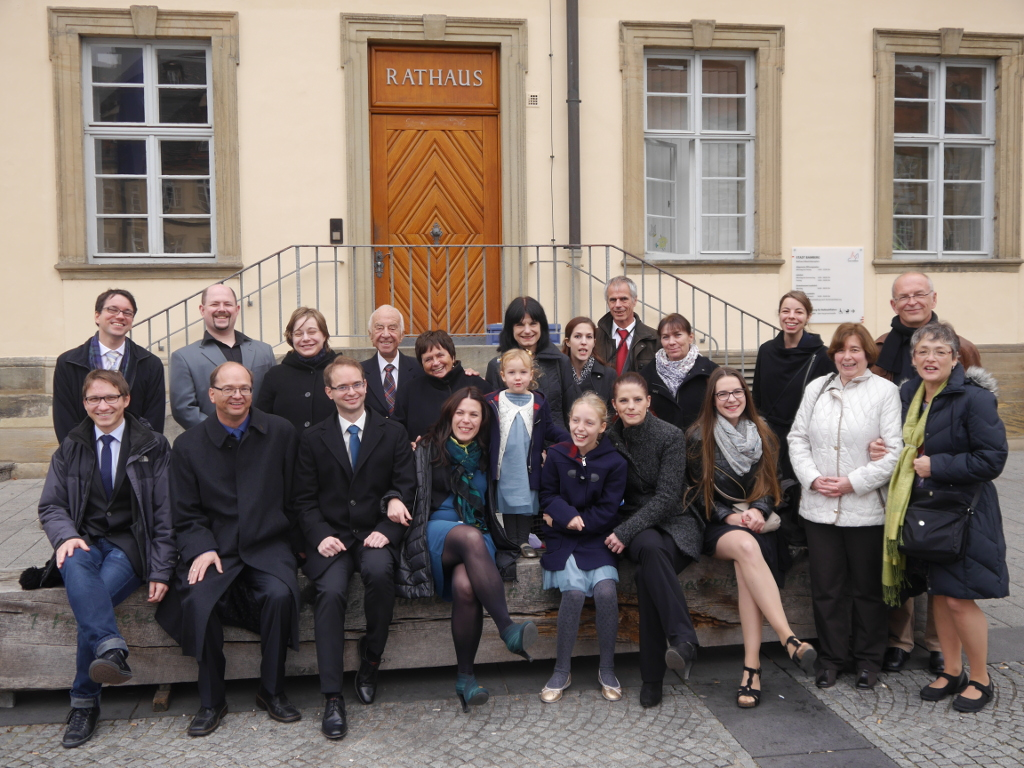
\includegraphics[width=\textwidth]{pic/front.jpg}
	\end{figure}
\LARGE
	\today
\end{titlepage}
\thispagestyle{empty}



\cleardoublepage
\tableofcontents


\cleardoublepage


% background graphic
%\setBackgroundPicture[x, y=-2cm, width=\paperwidth-4cm, height, orientation = pagecenter]{pic/background}

\begin{otherlanguage}{ngerman}
\setHeadlines
{% translation
    inghead = Zutaten,
    prephead = Zubereitung,
    hinthead = Tipp,
    continuationhead = Fortsetzung,
    continuationfoot = Fortsetzung auf n\"achster Seite,
    portionvalue = Personen,
}

%%%%%%%%%%%%%%%%%%%%%%%%%%%%%%%%%%%%%%%%%%%%%%%%%%%%%%%%%%%%%%%%%%%
%				Recipe Section										%
%%%%%%%%%%%%%%%%%%%%%%%%%%%%%%%%%%%%%%%%%%%%%%%%%%%%%%%%%%%%%%%%%%%
\cleardoublepage
\section{Vegetarische Speisen}
\begin{figure}[h]
	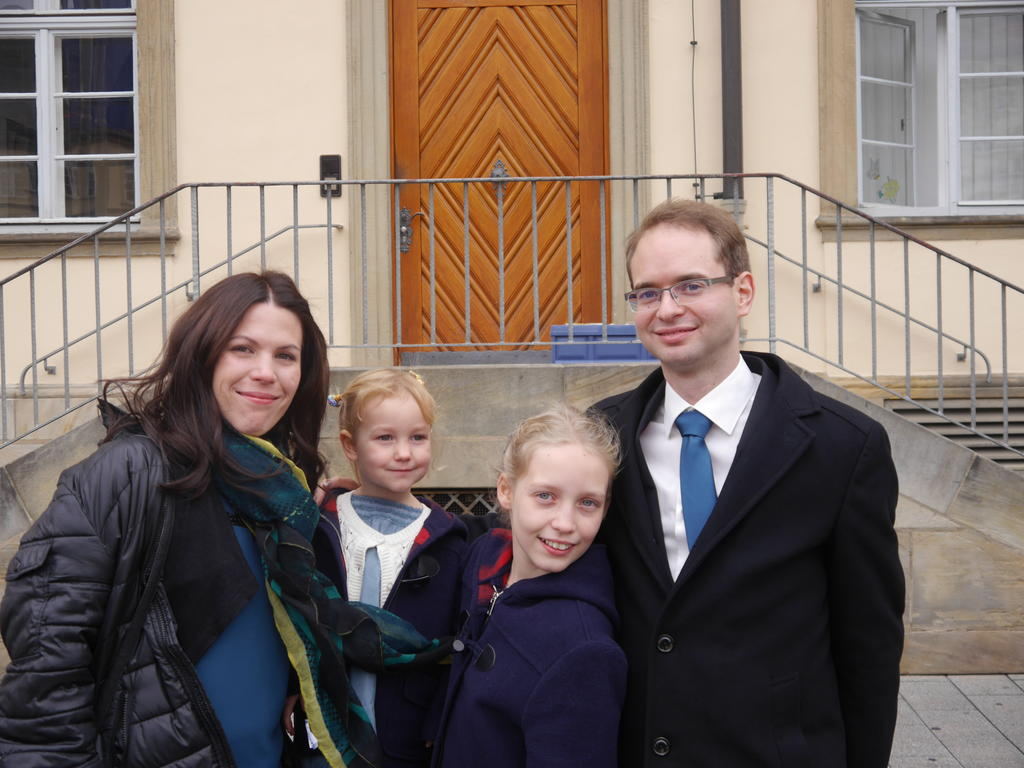
\includegraphics[width=\textwidth]{pic/veggie.jpg}
\end{figure}


\begin{recipe}
[% 
    preparationtime = {\unit[30]{min}},
    portion = {\portion{4}},
    source = {Lieblingsrezept von Ariane (original von chefkoch.de)}
]
{Ratatouille mit Tofu}

    \ingredients{%
        500 g	& 	Tomaten \\
		500 g	& 	Zucchini \\
		500 g &	Paprikaschoten \\
		500 g	&	Aubergine\\
		2	&	Zwiebeln \\
		2	&	Knoblauchzehen \\
		400 g & Räuchertofu \\
		4 EL & Olivenöl\\
		 & Salz und Pfeffer\\
		 2 Stiele & Thymian\\
		2 Stiele & Rosmarin\\
		2 Stiele & Oregano\\
		2 & Lorbeerblatt\\
    }
    
    \preparation{%
    \newline
       \step Das Gemüse gründlich waschen, die Tomaten häuten und in grobe Stücke schneiden. Die Zwiebeln schälen und wie das restliche Gemüse würfeln (ca. erbsengroß). Den Knoblauch schälen und fein hacken. 
       \step Das Olivenöl in einem weiten Topf erhitzen, die Gemüse darin getrennt nach Sorten jeweils 10 Minuten garen, dann herausnehmen (das Gemüse für das Ratatouille getrennt anbraten und erst ganz am Ende miteinander vermischen).
       \step Anschließend den Tofu kurz abtrocknen und würfeln. Das Gemüse vermengen. Die Kräuter mit dem Lorbeerblatt, dem Knoblauch und dem gewürfelten Tofu dazugeben. Mit Salz und Pfeffer würzen und alles weitere 10 Minuten garen.
    }
   
\end{recipe}

\cleardoublepage
\subsection{Herbstrezepte}
\begin{figure}[h]
	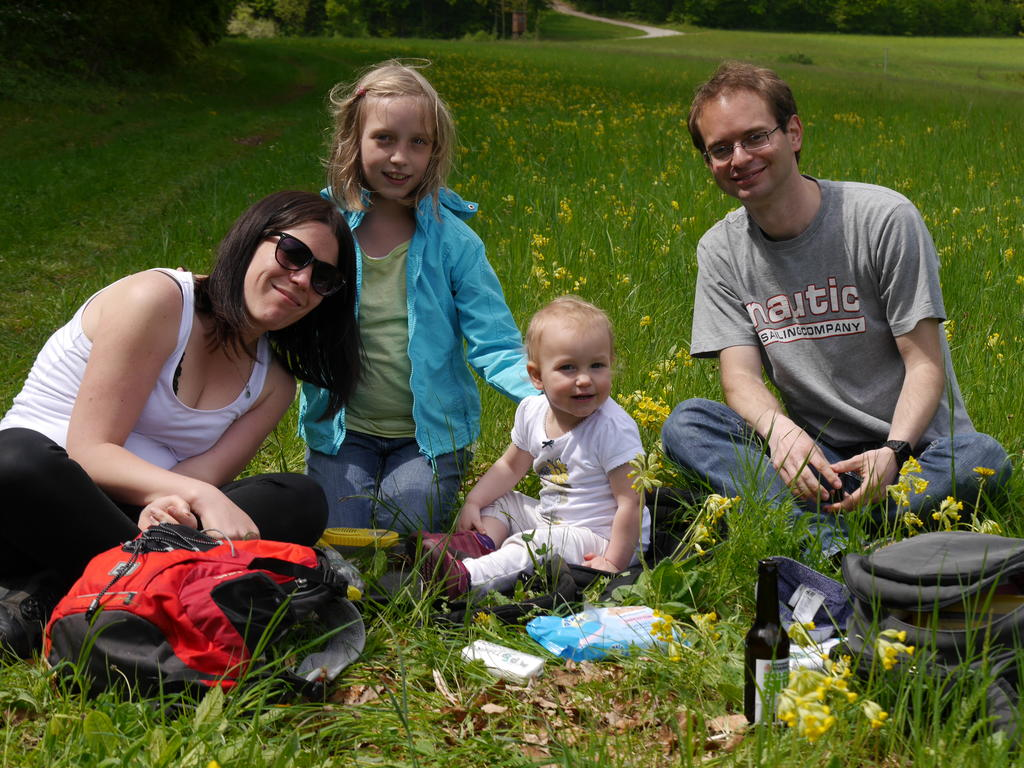
\includegraphics[width=\textwidth]{pic/US}
\end{figure}
% Complete recipe example
\begin{recipe}
[% 
    preparationtime = {\unit[40]{min}},
    %bakingtime={\unit[1]{h}},
    %bakingtemperature={\protect\bakingtemperature{
     %   fanoven=\unit[230]{\textcelcius},
     %   topbottomheat=\unit[195]{°C},
     %   topheat=\unit[195]{°C},
     %   gasstove=Level 2}},
    portion = {\portion{4}},
    %calory={\unit[3]{kJ}},
    source = {Köstlich Vegetarisch}
]
{Fruchtige Butternut-Kürbis-Suppe}
    
    \graph
    {% pictures
        %small=pic/PumpkinSoup,     % small picture
        big=pic/PumpkinSoup  % big picture
    }
    
    %\introduction{%
     %   \blindtext
    %}
    
    \ingredients{%
        1,2 kg	& 	Butternut-Kürbis \\
		250 g	& 	Äpfel (säuerlich) \\
		100    	&	Zwiebeln \\
		3 EL	&	Butter \\
		2 TL	&	Curry \\
		40 g	&	Weizenmehl \\
		1 Liter	&	Gemüsebrühe \\
		1 		&	Bio-Orange \\
 				&	Salz und Pfeffer\\
 				&	Muskat \\
 		4 EL	& 	Cr{\'e}me fra{\^i}che
    }
    
    \preparation{%
    \newline
       \step Kürbis vierteln, schälen, fasriges Gewebe und Kerne entfernen. Äpfel vierteln, schälen und Kerngehäuse entfernen und Zwiebel schälen. Alles 1\unitfrac{1}{2} cm groß würfeln.
       \step Butter in großen Topf zerlassen und Zwiebeln darin anschwitzen. Kürbis, Äpfel und Currypulver hinzugeben und unter Rühren 3 Minuten anbraten. Mit Mehl bestäuben und mit Gemüsebrühe angießen. 15-20 Minuten mit geschlossenem Topf auf mittlerer Hitze kochen.
       \step Inzwischen Orangen heiß abwaschen, trocken reiben und Schale fein abreiben; Saft auspressen und beides zur Suppe geben. Aufkochen lassen, fein pürieren und mit Gewürzen abschmecken.   
    }
    
    \suggestion[Servierbeispiel]
    {%
        Suppe auf Wunsch mit Cr{\'e}me fra{\^i}che garnieren und servieren.
    }
    
   % \suggestion{%
    %    \blindtext
   % }
    
    \hint{%
        Die Suppe erhält durch Zugabe von Schwarzkümmel einen pfeffrigen Geschmack ohne zusätzliche Schärfe.
    }
    
\end{recipe}
% Complete recipe example
\begin{recipe}
[% 
    preparationtime = {\unit[30]{min}},
    %bakingtime={\unit[1]{h}},
    %bakingtemperature={\protect\bakingtemperature{
     %   fanoven=\unit[230]{\textcelcius},
     %   topbottomheat=\unit[195]{°C},
     %   topheat=\unit[195]{°C},
     %   gasstove=Level 2}},
    portion = {\portion{5-6}},
    %calory={\unit[3]{kJ}},
    source = {Chefkoch}
]
{Grünkohl - Cremesüppchen}
    
    \graph
    {% pictures
        small=pic/CurlyKaleSoup2,     % small picture
        big=pic/CurlyKaleSoup  % big picture
    }
    
    %\introduction{%
     %   \blindtext
    %}
    
    \ingredients{%
        750 g	& 	Grünkohl\\
		350 g	& 	Kartoffeln\\
		1   	&	Zwiebel\\
		3 		&	Möhren\\
		1 Zehe	&	Knoblauch\\
		50 g	&	Butter\\
		1 EL	&	Cr{\`e}me fra{\^i}che\\
		1 Liter	&	kräftige Gemüsebrühe\\
 				&	Salz und Pfeffer\\
 				&	Muskat
    }
    
    \preparation{%
    \newline
        Den Grünkohl von den Rippen streifen, waschen, in Salzwasser blanchieren.
        Kartoffeln und Möhren schälen, grob würfeln. 
        Zwiebel würfeln und mit dem gehackten Knoblauch in Butter andünsten. Grünkohl, Möhren und Kartoffeln zugeben, kurz mitdünsten, dann Brühe zugeben und alles zusammen weich kochen lassen.
        Mit dem Pürierstab fein pürieren, Cr{\`e}me fra{\^i}che einrühren, dann mit Salz, Pfeffer und Muskat abschmecken.
        Man kann dazu Würstchen aller Art reichen.
        Eine schöne Variante ist auch, in die Teller ganz dünn geschnittenes, frisches Lachsfilet zu geben und die heiße Suppe dann darüber gießen.
    }
    
    %\suggestion[Headline]
    %{%
    %    \blindtext
   % }
    
   % \suggestion{%
    %    \blindtext
   % }
    
    \hint{%
        Die Grünkohlsuppe lässt sich mit Debrezinern gut ergänzen.
    }
    
\end{recipe}
% Complete recipe example
\begin{recipe}
[% 
    preparationtime = {\unit[50]{min}},
    %bakingtime={\unit[1]{h}},
    %bakingtemperature={\protect\bakingtemperature{
     %   fanoven=\unit[230]{\textcelcius},
     %   topbottomheat=\unit[195]{°C},
     %   topheat=\unit[195]{°C},
     %   gasstove=Level 2}},
    portion = {\portion{4}},
    %calory={\unit[3]{kJ}},
    source = {Köstlich Vegetarisch}
]
{Indischer-Linsen-Fenchel-Eintopf}
    
    \graph
    {% pictures
        %small=pic/CurlyKaleSoup2,     % small picture
        big=pic/LinsenFenchelEintopf  % big picture
    }
    
    %\introduction{%
     %   \blindtext
    %}
    
    \ingredients{%
        700 g	& 	Fenchel\\
		250 g	& 	Möhren\\
		1   	&	rote Chilischote\\
		2 		&	walnussgroße Stücke Ingwer\\
		2EL		&	Bratöl\\
		2EL		&	gelbe Senfkörner\\
		2EL		&	Kurkuma\\
		2EL		&	Curry\\
 		200g	&	Berglinsen\\
 		\unitfrac{1}{2}TL&	Zimt\\
 		200g	&	Basmatireis\\
 	\unitfrac{1}{2}Bund & Petersilie\\ 	
 				&	Salz und Pfeffer\\
    }
    
    \preparation{%
    \step Fenchel waschen, putzen, Fenchelgrün zur Seite legen, Knollen vierteln, Strunk entfernen und Viertel würfeln. Möhren ebenfalls würfeln. Chili waschen, der Länge nach halbieren, entkernen und fein würfeln. Ingwer schälen und klein hacken.
    \step Öl und Senfkörner in einem großen Topf leicht erhitzen, dabei Deckel drauflegen, die Senfkörner können springen. Ingwer und Chili zugeben und 1 Minute braten. Gemüse, Kurcuma und Curry zugeben, weitere 3 Minuten braten. Linsen und rund 600 ml Wasser zugeben. Zum Kochen bringen und im geschlossenem Topf auf kleiner Hitze ca 25 Minuten garen, bis Linsen weich aber noch bissfest sind. Mit Salz und Zimt würzen und 3-4 minuten durchziehen lassen.
    \step Inzwischen Reis nach Packunganleitung (in der Regel mit doppelter Menge Wasser) gar kochen. Fenchelgrün und Petersilie abrausen, trockenschütteln und fein hacken. Linsen-Fenchel-Eintopf mit Reis und Kräutern gariert servieren.
    }
    
    %\suggestion[Headline]
    %{%
    %    \blindtext
   % }
    
   % \suggestion{%
    %    \blindtext
   % }
    
    \hint{%
       Auch lecker: Am Ende noch ein paar Organgenscheiben unterheben und Curry mit Orangensaft abschmecken.
    }
    
\end{recipe}
% Complete recipe example
\begin{recipe}
[% 
    preparationtime = {\unit[80]{min}},
    %bakingtime={\unit[1]{h}},
    %bakingtemperature={\protect\bakingtemperature{
     %   fanoven=\unit[230]{\textcelcius},
     %   topbottomheat=\unit[195]{°C},
     %   topheat=\unit[195]{°C},
     %   gasstove=Level 2}},
    portion = {\portion{4}},
    %calory={\unit[3]{kJ}},
    source = {Vegetarisch Köstlich}
]
{Tomatentopf mit Seitanwürfeln und gelbem Würzreis}
    
    \graph
    {% pictures
       % small=pic/CurlyKaleSoup2,     % small picture
        big=pic/TomatoeBredie  % big picture
    }
    
    %\introduction{%
     %   \blindtext
    %}
    
    \ingredients{%
        100 g		& 	Zwiebeln \\
		3 Zehen		& 	Knoblauch \\
		300 g  		&	festkochenende Kartoffeln \\
		500 g		&	Tomaten\\
		200 g		&	weiße Bohnen \\
		1 Bund 		&	Majoran \\
		3 EL		&	Öl \\
		2 EL		&	Tomatenmark \\
		1 TL		&	Zucker \\
 		1 TL		&	Paprikapulver \\
 		1 Msp		& 	Chilipulver	\\
 		350 ml 		& 	Gemüsebrühe \\
 		200 g		&	Seitan \\
 		200 g		& paraboiled Reis\\
 		60 g		& Rosinen\\
 		1 TL		& Kurkuma\\
 		1			& Zimtstange
    }
    
    \preparation{%
       \step Zwiebeln und Knoblauch fein würfeln. Kartoffeln schälen, Tomaten waschen und beide 1\unitfrac{1}{2}cm groß würfeln. Öl in großem Topf erhitzen, Zwiebeln darin bei mittlerer Hitze ca. 4 Minuten goldgelb anrbaten. Tomatenmark und Knoblauch zugeben und 3 Minuten unter Rühren mitbraten. Tomaten, Kartoffeln, Bohnen, Majoran,  Zucker, 1TL Salz, Paprikapulver, Chilipulver und Gemüsebrühe hinzugeben und 50 Minuten bei mittlerer Hitze im offenen Topf dicklich einkochen lassen. Zwischendurch umrühren.
       \step Inzwischen den Reis nach Packungsanleitung mit Rosinen, Kurkuma, Zimtstange und Salz zubereiten. Ggf. restliche Flüssigkeit abgießen und Zimstange entfernen.
       \step Seitan 1cm groß würfeln und in einer Pfanne mit restlichem Öl ca. 5-7 Minuten kross anbraten. Zum Tomatentopf geben und alles mit Salz und Pfeffer anbraten.
   
    }
    
    \suggestion
    {%
           Traditionell wird dieser Topf mit Lamm oder Hammelfleisch gekocht und ist ein südafrikanisches Gericht. Je länger der Eintopf simmert und zieht desto intensiver schmeckt er, hierfür kann man auch getrocknete Bohnen verwenden und die Kochzeit dementsprechend erhöhen. 
    }
    
   % \suggestion{%
    %    \blindtext
   % }
    
    
\end{recipe}
% Complete recipe example
\begin{recipe}
[% 
    preparationtime = {\unit[40]{min}},
    %bakingtime={\unit[1]{h}},
    %bakingtemperature={\protect\bakingtemperature{
     %   fanoven=\unit[230]{\textcelcius},
     %   topbottomheat=\unit[195]{°C},
     %   topheat=\unit[195]{°C},
     %   gasstove=Level 2}},
    portion = {\portion{4}},
    %calory={\unit[3]{kJ}},
    %source = {Vegetarisch Köstlich}
]
{Brokkoli Sugo}
    
    \graph
    {% pictures
       % small=pic/BroccoliNoodles2,     % small picture
        big=pic/BroccoliNoodles  % big picture
    }
    
    %\introduction{%
     %   \blindtext
    %}
    
    \ingredients{%
       500 g					& 	Brokkoli \\
		3 						& 	Zwiebeln \\
		1	  					&	Knoblauch \\
		300 g					&	Tomaten\\
		5						&	getrocknete Tomaten\\
			 					&	Kapern \\
		2 EL					&	Öl \\
		2 EL					&	Tomatenmark \\
		\unitfrac{1}{2} TL		&	Zucker \\
 		1 TL					&	Paprikapulver \\
 		\unitfrac{1}{2}			&	Limette \\	
 		300 g					&	Nudeln
    }
    
    \preparation{%
    	\step Brokkoli putzen, in kleine Röschen zerteilen, dicke Stiele schälen und in kleine Stücke schneiden, alles waschen. Salzwasser in Topf zum Kochen bringen und Stiele darin 3 Minuten blanchieren. Die Hälfte der Röschen zugeben und weitere 3 Minuten blanchieren danach abgießen und gut abtropfen lassen.
    	\step In der Zwischenzeit Knoblauch und Zwiebeln schälen und würfeln. Tomaten, getrocknete Tomaten würfeln. Öl in einem Topf erhitzen und Knoblauch und Zwiebeln unter rühren anbraten und mit Gemüsebrühe ablöschen. Restlichen Brokkoli, Tomaten, Kapern hinzugeben bei mittlerer Hitze zugedeck weichgaren.
    	\step In der Zwischenzeit Nudeln nach Packungsanleitung zubereiten.
    	\step Brokkoli Sugo mit dem Pürierstab pürieren, mit Gewürzenund Limettensaft abschmecken. Nudeln abgießen mit Sugo und Brokkoliröschen mischen und servieren.
   	
       	}
       
       
        \hint{%
        Gerne noch mit Parmesan oder Morzarella bestreuen. Alternativ: Cashewkerne im Mixer hacken und mit Hefeflocken mischen. 
   		}
       	

\end{recipe}
% Complete recipe example
\begin{recipe}
[% 
    preparationtime = {\unit[30]{min}},
    %bakingtime={\unit[1]{h}},
    %bakingtemperature={\protect\bakingtemperature{
     %   fanoven=\unit[230]{\textcelcius},
     %   topbottomheat=\unit[195]{°C},
     %   topheat=\unit[195]{°C},
     %   gasstove=Level 2}},
    portion = {\portion{4}},
    %calory={\unit[3]{kJ}},
    source = {Vegetarisch Köstlich}
]
{Champignon-Zucchini-Pfanne}
    
    \graph
    {% pictures
        small=pic/ChampignonZucchiniPfanne,     % small picture
        big=pic/ChampignonZucchiniPfanne2  % big picture
    }
    
    %\introduction{%
     %   \blindtext
    %}
    
    \ingredients{%
     \textbf{Polenta:}			& 	 \\
    	750 ml					& 	Gemüsebrühe \\
		450 ml 					& 	Milch \\
		1	  					&	Lorbeerblatt \\
		180 g					&	Polenta\\
		30	g					&	Parmesan\\
		30	g					&	Butter\\
		\textbf{Pfanne:}		& 	 \\
		200 g					&	Zwiebeln \\
		1						&	Knoblauchzehe \\
		\unitfrac{1}{2} Bund	&	Petersilie \\
 		600 g					&	braune Champignons \\
 		3 EL					&	Olivenöl \\	
 		2 TL					&	Majoran \\
 		3 EL					&	dunkler Balsamico-Essig\\
 		 						&	Salz und Pfeffer
    }
    
    \preparation{%
    	\step Für die Polenta Brühe, Milch und Lorbeerblatt in Topf aufkochen. Polenta unter Rühren einstreuen, kurz aufkochen lassen und im geschlossenen Topf bei kleinster Hitze ca. 20 Minuten quellen lassen, dabei gelegentlich umrühren. Parmesan fein reiben.
    	\step In der Zwischenzeit für die Champignon-Pfanne Knoblauch und Zwiebeln schälen und würfeln. Petersilie abbrausen, trocken schütteln und fein hacken. Champignons putzen und halbieren oder vierteln. Zucchini waschen und fein würfeln.
    	\step Olivenöl in einer großen Pfanne erhitzen und Knoblauch, Zwiebeln darin ca. 3 Minuten anschwitzen. Champignons und Zuchhini dazugeben und ca. 5 Minuten braten. Majoran, Salz und Pfeffer würzen. Mit Balsamico ablöschen, Petersilie unterühren.
    	\step Polenta mit Salz und Pfeffer abschmecken, Lorbeerblatt entfernen, Butter einrühren. Parmesan unterühren. Polenta mit Gemüse servieren.   	
       	}
       
       
        \hint{%
       Die Polenta ist auch toll mit 1,2 l Gemüsebrühe, ohne Parmesan und mit 4 EL Olivenöl verfeinern.
   		}
       	

\end{recipe}
% Complete recipe example
\begin{recipe}
[% 
    preparationtime = {\unit[30]{min}},
    %bakingtime={\unit[1]{h}},
    %bakingtemperature={\protect\bakingtemperature{
     %   fanoven=\unit[230]{\textcelcius},
     %   topbottomheat=\unit[195]{°C},
     %   topheat=\unit[195]{°C},
     %   gasstove=Level 2}},
    portion = {\portion{3-4}},
    %calory={\unit[3]{kJ}},
    source = {Wok}
]
{Weißkohlwok mit Ananas und Paprika}
    
    \graph
    {% pictures
       % small=pic/CurlyKaleSoup2,     % small picture
        big=pic/ColeSlawWok  % big picture
    }
    
    %\introduction{%
     %   \blindtext
    %}
    
    \ingredients{%
        500 g		& 	Weißkohl \\
		1			& 	rote Paprika \\
		200 g  		&	Ananas \\
		1 Stängel	&	Zitronengras \\
		1 			&	Chilischote \\
		200	g		&	(Mungobohnen-) Sprossen \\
		2 EL		&	Sojasauce \\
		4 EL		&	Sherry \\
 					&	Salz und Pfeffer \\
 		1 TL		&	Speisestärke \\
 		2 EL		& 	Kokosraspel	\\
 		1 EL 		& 	weiße Sesamsamen \\
 		\unitfrac{1}{2} TL & Zitronenschale \\
 		4 EL		& 	Öl 
    }
    
    \preparation{%
       \step Den Kohl und die Paprika waschen, putzen und in feine Streifen schneiden. Die Ananas schälen, den Strunk entfernen und in Stücke schneiden. Zitronengras putzen, waschen und die Zwiebel hacken. Chilischote halbieren, entkernen und in feine Scheiben schneiden. Sprossen in einem Sieb abbrausen und abtropfen lassen.
       \step Sojasauce, Sherry, Salz und Pfeffer zu einer Sauce verquirlen.
       \step Kokosraspeln und Sesam im Wok ohne Fett goldgelb rösten.
       \step Den Wok mit Öl erhitzen. Kohl- und Paprikstreifen unter Rühren bissfest garen. Ananas, Zitronengras, Chilischote und Sprossen hinzugeben; die Saucenmischung unterrühren. Etwa 2 Minuten garen lassen und mit Kokosraspel-Sesam-Mischung und Zitronenschalen bestreuen.
   
    }
    
    %\suggestion[Headline]
    %{%
    %    \blindtext
   % }
    
   % \suggestion{%
    %    \blindtext
   % }
    
    \hint{%
        Eine Messerspitze Bockshornkleesamen macht das Gericht bekömmlicher.
    }
    
\end{recipe}
% Complete recipe example
\begin{recipe}
[% 
    preparationtime = {\unit[50]{min}},
    bakingtime={\unit[40]{min}},
    bakingtemperature={\protect\bakingtemperature{
        fanoven=\unit[160]{\textcelcius},
        topbottomheat=\unit[180]{\textcelcius},
        %topheat=\unit[195]{°C},
        %gasstove=Level 2}
        }},
    portion = {\portion{4}},
    %calory={\unit[3]{kJ}},
    source = {Köstlich Vegetarisch}
]
{Brokkoli-Süßkartoffel-Auflauf mit\\[.5ex] Quinoa-Haube}
    
    \graph
    {% pictures
        small=pic/BrokkoliMitQuinoaHaube,     % small picture
        big=pic/BrokkoliMitQuinoaHaube2  % big picture
    }
    
    %\introduction{%
     %   \blindtext
    %}
    
    \ingredients{%
        150 g	& 	bunte oder helle Quinoa\\
		600 g	& 	Brokkoli\\
		500 g  	&	Süßkartoffeln\\
		2 		&	Knoblauchzehen\\
		1		&	Zwiebel\\
		10		&	Salbeiblätter\\
		4 EL	&	Olivenöl\\
		1 TL	&	Zucker\\
 		\unitfrac{1}{2} Bund & Petersilie\\
 		100 g	&	Parmesan\\
 		3		&	Eier\\
 				&	Muskat\\
 	\unitfrac{1}{2} TL & Chili\\ 	
 				&	Salz und Pfeffer\\
    }
    
    \preparation{%
    \step Quinoa in Sieb kalt abrausen. In reichlich Salzwasser ca. 18 Minuten bei kleiner Hitze im halb offenen Topf garen. Abgießen abtropfen und lassen.
    \step Inzwischen Brokkoli putzen, in kleine Röschen zerteilen, dicke Stiele schälen und in kleine Stücke schneiden, alles waschen. Salzwasser in Topf zum Kochen bringen und Stiele darin 3 Minuten blanchieren. Röschen zugeben und weitere 3 Minuten blanchieren danach abgießen und gut abtropfen lassen. Süßkartoffeln schälen und würfeln.
    \step Knoblauch und Zwiebeln schälen und würfeln. Salbeiblätter kalt abbrausen, tocken schütteln und in feine Streifen schneiden. Öl in Pfanne erhitzen und Knoblauch, Zwiebeln und Salbei unter Rühren darin ca. 3 Minuten anbraten. Süßkartoffeln und Zucker zugeben und weitere 3 Minuten anbraten. Mit 150ml Wasser ablöschen und weitere 10 Minuten garen (bis Wasser verdampft ist). Etwas abkühlen lassen und mit Brokkoli in einer Auflaufform vermischen. Petersilie abrausen, trocken schütteln, fein hacken und ebenfalls unterheben. Mit Salz und Pfeffer würzen.
    \step Backofen vorheizen. Käse reiben. Eier mit Schneebesen verquirlen und mit Käse zu Quinoa geben. Mit Salz, Muskat und Chili würzen und gut vermischen. Quinoamasse auf Gemüse verteilen und  ca. 35-40 Minuten backen und warm servieren.
    }
    
    %\suggestion[Headline]
    %{%
    %    \blindtext
   % }
    
   % \suggestion{%
    %    \blindtext
   % }
    
  
    
\end{recipe}
% Complete recipe example
\begin{recipe}
[% 
    preparationtime = {\unit[30]{min}},
    bakingtime={\unit[10]{min}},
    %bakingtemperature={\protect\bakingtemperature{
     %   fanoven=\unit[230]{\textcelcius},
     %   topbottomheat=\unit[195]{°C},
     %   topheat=\unit[195]{°C},
     %   gasstove=Level 2}},
    portion = {\portion{5-6}},
    %calory={\unit[3]{kJ}},
    source = {Chefkoch}
]
{Käsefondue}
    
    \graph
    {% pictures
        small=pic/Cheese,     % small picture
        big=pic/AmelieCheese  % big picture
    }
    
    %\introduction{%
     %   \blindtext
    %}
    
    \ingredients{%
    	4						& 	Baguette \\
    	300 g					& 	Appenzeller \\
    	300 g					& 	Bergkäse \\
    	300 g					& 	Emmentaler \\
      	300 g					& 	Gruy{\'e}re \\
		1 Flasche 				&	Weißwein \\
		2 TL 	 				&	Speisestärke \\
		\unitfrac{1}{2} TL		&	Natron \\
		4 cl					&	Kirschwasser \\
								&	Pfeffer \\
		2 Msp.					& 	Paprikapulver \\
		2 Msp.					&	Muskat \\
		1 Zehe					&	Knoblauch \\
    }
    
    \preparation{%
    \step Den Fonduetopf mit der einen Hälfte des Knoblauchs ausreiben.
    \step Wein in den Topf gießen und bei kleiner Hitze langsam erwärmen. 
    \step Ist der Wein heiß, den Käse portionsweise hineingeben und unter ständigem Rühren schmelzen lassen.
    \step Die andere Hälfte der Knoblauchzehe pressen und zum Käse geben. 
    \step Die Speisestärke mit dem Kirschwasser verrühren, zum Käse geben und unter Rühren noch mal aufkochen lassen. Das Fondue mit Pfeffer, Paprika und Muskat würzen und Natron hinzugeben.
    }
    
    \suggestion[Am Tisch]{%
        Die Flamme im Rechaud entzünden.	
		Baguettestücke auf Fonduegabeln spießen, in das Fondue eintauchen und genießen.   
    }
    
   % \suggestion{%
    %    \blindtext
   % }
    
    \hint{%
        Zusätzlich zu Baguette können auch Weintrauben, Ananas und Paprika gereicht werden.
    }
    
\end{recipe}
% Complete recipe example
\begin{recipe}
[% 
    preparationtime = {\unit[80]{min}},
    %bakingtime={\unit[1]{h}},
    %bakingtemperature={\protect\bakingtemperature{
     %   fanoven=\unit[230]{\textcelcius},
     %   topbottomheat=\unit[195]{°C},
     %   topheat=\unit[195]{°C},
     %   gasstove=Level 2}},
    portion = {\portion{2-3}},
    %calory={\unit[3]{kJ}},
    source = {Vegetarisch Köstlich}
]
{Avocado-Mousse au Chocolat:}
    
    \graph
    {% pictures
       % small=pic/CurlyKaleSoup2,     % small picture
        big=pic/AvocadoMouse  % big picture
    }
    
    %\introduction{%
     %   \blindtext
    %}
    
    \ingredients{%
        2		& 	Avocado \\
		1		& 	Banane \\
		5 EL 	&	Kakao \\
		1 EL 	&	Agavendicksaft\\
    }
    
    \preparation{%
       \step Avocados schälen und Kern entfernen. Avocados grob kleinschneiden und in einen Mixer oder eine Schüssel geben.
       \step Kakao und Agavendicksaft hinzugeben.
       \step Alles im Mixer oder mit dem Stabmixer pürieren.
   
    }
    
    \hint
    {%
        Eine andere Variante benutzt Cashewkerne: 1 Tasse Cashewkerne mindestens 1 Stunde einweichen, Kerne nach dem Einweichen in den Mixer und mit 1 TL Agavendicksaft, 4 TL Kokosöl, \unitfrac{1}{2} TL Vanille, etwas Wasser und 3 TL Kakao mixen.
    }
    
   % \suggestion{%
    %    \blindtext
   % }
    
    
\end{recipe}


\end{otherlanguage}

\clearpage
~\thispagestyle{empty}
% Last page
\clearpage
\thispagestyle{empty}
~
\vfill
\begin{center}
\begin{tikzpicture}[scale=1.5]
\fill (0,0) -- (-0.2, 0.1) -- (-4, 0) -- (-0.2, -0.1) -- cycle;
\fill (0,0) -- (0.2, 0.1) -- (4, 0) -- (0.2, -0.1) -- cycle;
\fill (0,0) circle (0.1);
\end{tikzpicture}
\end{center}


    Eine hochzeitliche Rezeptesammlung -- Gerichte die wir G"aste lecker finden! Wir hoffen ihr findet die eine oder andere Anregung und denkt beim Kochen und Genießen an uns und das wundersch"one Fest.
    
    Wenn ihr mal ausgeschlafen habt könnt ihr unsere ganzen pull-requests unter \url{https://github.com/whatever4711/cookbook} annehmen.
\end{document} 